\documentclass[letterpaper,USenglish,cleveref, autoref, thm-restate]{lipics-v2021}
%This is a template for producing LIPIcs articles.
%See lipics-v2021-authors-guidelines.pdf for further information.
%for A4 paper format use option "a4paper", for US-letter use option "letterpaper"
%for british hyphenation rules use option "UKenglish", for american hyphenation rules use option "USenglish"
%for section-numbered lemmas etc., use "numberwithinsect"
%for enabling cleveref support, use "cleveref"
%for enabling autoref support, use "autoref"
%for anonymousing the authors (e.g. for double-blind review), add "anonymous"
%for enabling thm-restate support, use "thm-restate"
%for enabling a two-column layout for the author/affilation part (only applicable for > 6 authors), use "authorcolumns"
%for producing a PDF according the PDF/A standard, add "pdfa"

%\pdfoutput=1 %uncomment to ensure pdflatex processing (mandatatory e.g. to submit to arXiv)
%\hideLIPIcs  %uncomment to remove references to LIPIcs series (logo, DOI, ...), e.g. when preparing a pre-final version to be uploaded to arXiv or another public repository

%\graphicspath{{./graphics/}}%helpful if your graphic files are in another directory

\usepackage{amsmath}
\usepackage{tikz}
\usepackage{pgfplots}
\usepackage{booktabs}
\usepackage{hyperref}

\newcommand{\pand}{\mathbin{\land^{\sf p}}}
\newcommand{\por}{\mathbin{\lor^{\sf p}}}
\DeclareMathOperator*{\Pand}{\bigwedge^{\sf p}}
\DeclareMathOperator*{\Por}{\bigvee^{\sf p}}
\newcommand{\boolnot}{\neg}
\newcommand{\tautology}{\top}
\newcommand{\nil}{\bot}
\newcommand{\obar}[1]{\overline{#1}}
\newcommand{\oneminus}{{\sim}}
\newcommand{\lit}{\ell}

\newcommand{\varset}{X}
\newcommand{\exvarset}{Z}
\newcommand{\dependencyset}{{\cal D}}
\newcommand{\litset}{{\cal L}}
\newcommand{\ring}{{\cal R}}
\newcommand{\dset}{{\cal A}}
\newcommand{\rep}{\textbf{R}}
\newcommand{\radd}{+}
\newcommand{\rmul}{\times}
\newcommand{\addident}{\textbf{0}}
\newcommand{\mulident}{\textbf{1}}
\newcommand{\imply}{\Rightarrow}
\newcommand{\ifandonlyif}{\Leftrightarrow}
\newcommand{\drational}{\mathbb{Q}_{2,5}}

\newcommand{\assign}{\alpha}
\newcommand{\passign}{\rho}
\newcommand{\lassign}{\beta}
\newcommand{\uassign}{{\cal U}}
\newcommand{\modelset}{{\cal M}}

\newcommand{\indegree}{\textrm{indegree}}
\newcommand{\outdegree}{\textrm{outdegree}}
\newcommand{\validate}{\textsf{validate}}
\newcommand{\prov}{\textrm{Prov}}
\newcommand{\inputformula}{\phi_I}
\newcommand{\pogformula}{\phi_P}

\newcommand{\makenode}[1]{\mathbf{#1}}
\newcommand{\nodeu}{\makenode{u}}
\newcommand{\nodev}{\makenode{v}}
\newcommand{\nodes}{\makenode{s}}
\newcommand{\nodep}{\makenode{p}}
\newcommand{\noder}{\makenode{r}}

\newcommand{\simplify}[2]{#1|_{#2}}

\newcommand{\progname}[1]{\textsc{#1}}
\newcommand{\dfour}{\progname{D4}}
\newcommand{\Dfour}{\progname{D4}}
\newcommand{\cadical}{\progname{CaDiCal}}
\newcommand{\dtrim}{\progname{drat-trim}}

\definecolor{redorange}{rgb}{0.878431, 0.235294, 0.192157}
\definecolor{lightblue}{rgb}{0.552941, 0.72549, 0.792157}
\definecolor{clearyellow}{rgb}{0.964706, 0.745098, 0}
\definecolor{clearorange}{rgb}{0.917647, 0.462745, 0}
\definecolor{mildgray}{rgb}{0.54902, 0.509804, 0.47451}
\definecolor{softblue}{rgb}{0.643137, 0.858824, 0.909804}
\definecolor{bluegray}{rgb}{0.141176, 0.313725, 0.603922}
\definecolor{lightgreen}{rgb}{0.709804, 0.741176, 0}
\definecolor{darkgreen}{rgb}{0.152941, 0.576471, 0.172549}
\definecolor{redpurple}{rgb}{0.835294, 0, 0.196078}
\definecolor{midblue}{rgb}{0, 0.592157, 0.662745}
\definecolor{clearpurple}{rgb}{0.67451, 0.0784314, 0.352941}
\definecolor{browngreen}{rgb}{0.333333, 0.313725, 0.145098}
\definecolor{darkestpurple}{rgb}{0.396078, 0.113725, 0.196078}
\definecolor{greypurple}{rgb}{0.294118, 0.219608, 0.298039}
\definecolor{darkturquoise}{rgb}{0, 0.239216, 0.298039}
\definecolor{darkbrown}{rgb}{0.305882, 0.211765, 0.160784}
\definecolor{midgreen}{rgb}{0.560784, 0.6, 0.243137}
\definecolor{darkred}{rgb}{0.576471, 0.152941, 0.172549}
\definecolor{darkpurple}{rgb}{0.313725, 0.027451, 0.470588}
\definecolor{darkestblue}{rgb}{0, 0.156863, 0.333333}
\definecolor{lightpurple}{rgb}{0.776471, 0.690196, 0.737255}
\definecolor{softgreen}{rgb}{0.733333, 0.772549, 0.572549}
\definecolor{offwhite}{rgb}{0.839216, 0.823529, 0.768627}
\definecolor{medgreen}{rgb}{0.15, 0.6, 0.15}

% Lean code:
\usepackage{listings}
\definecolor{keywordcolor}{rgb}{0.7, 0.1, 0.1}   % red
\definecolor{tacticcolor}{rgb}{0.0, 0.1, 0.6}    % blue
\definecolor{commentcolor}{rgb}{0.4, 0.4, 0.4}   % grey
\definecolor{symbolcolor}{rgb}{0.0, 0.1, 0.6}    % blue
\definecolor{sortcolor}{rgb}{0.1, 0.5, 0.1}      % green
\definecolor{attributecolor}{rgb}{0.7, 0.1, 0.1} % red
\def\lstlanguagefiles{lstlean.tex}
% set default language
\lstset{language=lean, xleftmargin=1em}
\lstset{backgroundcolor=\color{white}}

\bibliographystyle{plainurl}% the mandatory bibstyle

\title{Certified Knowledge Compilation \\ with Application to Verified Model Counting}

\titlerunning{Certified Knowledge Compilation}

\author{Randal E. Bryant}{Computer Science Department, Carnegie Mellon University, Pittsburgh, PA 15213 USA}{rebryant@cmu.edu}{https://orcid.org/0000-0001-5024-6613}{Supported by NSF grant CCF-2108521}
\author{Wojciech Nawrocki}{Department of Philosophy, Carnegie Mellon University}{wjnawrock@cmu.edu}{https://orcid.org/0000-0002-8839-0618}{}
\author{Jeremy Avigad}{Department of Philosophy, Carnegie Mellon University}{avigad@cmu.edu}{https://orcid.org/0000-0003-1275-315X}{}
\author{Marijn J. H. Heule}{Computer Science Department, Carnegie Mellon University}{marijn@cmu.edu}{https://orcid.org/0000-0002-5587-8801}{Supported by NSF grant CCF-2108521}

\authorrunning{R. E. Bryant, et al} %TODO mandatory. First: Use abbreviated first/middle names. Second (only in severe cases): Use first author plus 'et al.'

%\Copyright{Jane Open Access and Joan R. Public} %TODO mandatory, please use full first names. LIPIcs license is "CC-BY";  http://creativecommons.org/licenses/by/3.0/

%\ccsdesc[100]{\textcolor{red}{Replace ccsdesc macro with valid one}} %TODO mandatory: Please choose ACM 2012 classifications from https://dl.acm.org/ccs/ccs_flat.cfm

%\keywords{Dummy keyword} %TODO mandatory; please add comma-separated list of keywords

%\category{} %optional, e.g. invited paper

%\funding{(Optional) general funding statement \dots}%optional, to capture a funding statement, which applies to all authors. Please enter author specific funding statements as fifth argument of the \author macro.

%\nolinenumbers %uncomment to disable line numbering

%Editor-only macros:: begin (do not touch as author)%%%%%%%%%%%%%%%%%%%%%%%%%%%%%%%%%%
%\EventEditors{John Q. Open and Joan R. Access}
%\EventNoEds{2}
%\EventLongTitle{42nd Conference on Very Important Topics (CVIT 2016)}
%\EventShortTitle{CVIT 2016}
%\EventAcronym{CVIT}
%\EventYear{2016}
%\EventDate{December 24--27, 2016}
%\EventLocation{Little Whinging, United Kingdom}
%\EventLogo{}
%\SeriesVolume{42}
%\ArticleNo{23}
%%%%%%%%%%%%%%%%%%%%%%%%%%%%%%%%%%%%%%%%%%%%%%%%%%%%%%

\newcommand{\program}[1]{\textsc{#1}}
\newcommand{\lean}{Lean~4}

\begin{document}

\maketitle

\begin{abstract}

\emph{Knowledge compilation} is the process of converting a Boolean
formula into a form that makes it possible to calculate associated
values efficiently, such as the weighted or unweighted model
count. Existing knowledge compilers, however,
provide no guarantee that the representation they generate
is logically equivalent to the original formula, and therefore they cannot validate the generated counts.

We present \emph{Partitioned Operation Graphs} (POGs), a generalization
of representations commonly used in knowledge compilation.
We have designed a proof framework that can prove the equivalence of a
POG representation with a Boolean formula in conjunctive normal form (CNF),
the standard input format for SAT solvers and model counting tools.

We have developed a program that can generate POG representations from
the d-DNNF graphs generated by the state-of-the-art knowledge compiler
\dfour, as well as independently checkable proofs that the output POGs
are equivalent to the input CNF formulas.  We have implemented an
efficient checker that can handle very large proofs. Our tool chain
for generating and verifying POGs scales to all but the largest d-DNNF
graphs generated by \dfour{} for formulas from a recent model counting
competition. Moreover, we present a checker and a model counter for POGs that have
been formally verified in the \lean{} proof assistant, thereby
creating the first formally verified toolchain for
weighted and unweighted
model counting.
\end{abstract}

\section{Introduction}

Modern Boolean satisfiability (SAT) solvers provide the ability to
find a satisfying assignment to a Boolean formula or to prove that no
such assignment exists.  They have applications across a variety of
domains, including formal verification of hardware, software, and
security protocols, computational mathematics, and combinatorial
optimization.  Some problems of interest, however, require going
beyond standard Boolean satisfiability.  For example, the {\em model
  counting problem} requires computing the number of satisfying
assignments of a formula, including in cases where there are far too many
to enumerate individually.  Model counting, in turn, has
applications in artificial intelligence, computer security, and
statistical sampling.  There are also many useful extensions of standard model counting,
including {\em
  weighted model counting}, where a weight is defined for
each possible assignment, and the goal becomes to compute the sum of the weights
of the satisfying assignments.

Model counting is a challenging problem---more challenging that the
already NP-hard problem of Boolean (un)satisfiability.  Several
tractable variants of Boolean satisfiability, including 2-SAT, become
intractable when the goal becomes model counting and not just
satisfiability \cite{valiant:siam:1979}.  Nonetheless, a number of
model counters have developed that scale to very large formulas, as
witnessed by their progress in the annual model counting competitions.

One approach to model counting, known as {\em knowledge compilation},
transforms the formula into a structured form for which model counting
becomes straightforward.  For example, the {\em deterministic,
  decomposable, negation normal form} (d-DNNF) introduced by
Darwiche~\cite{darwiche:aaai:2002,darwiche:ecai:2004} represents a
Boolean formula as a directed acyclic graph, with terminal nodes
labeled by Boolean variables and their complements, and with each
nonterminal node labeled by Boolean operation And or Or.  Restrictions
are placed on the structure of the graph such that a count of the
models can be computed by a single bottom-up traversal of the graph.
Kimmig, et al., present a very general framework, known as {\em
  algebraic model counting}~\cite{kimmig:jal:2017}, describing
properties of Boolean functions that can be efficiently computing from
its d-DNNF representation.  These include standard and weighted model
counting, and much more.

One shortcoming of existing knowledge compilers is that they have no
way to validate that their generated results are correct, i.e., that
the compiled representation is logically equivalent to the original
formula.  By contrast, all modern SAT solvers can generate
checkable proofs when they encounter unsatisfiable formulas.  The
guarantee provided by a checkable certificate of correctness enables
users of SAT solvers to fully trust their results.  Experience has also
shown that having this capability gives developers the ability quickly
detect and identify bugs in their solvers, and this, in turn, has led
to more reliable SAT solvers.

In this paper, we present \emph{Partitioned Operation Graphs} (POGs),
a generalization of the representations commonly used in knowledge
compilation, including d-DNNF\@.  We present the CRAT file format.
It captures both the structure of a POG and a checkable proof
that the POG is logically equivalent to a Boolean formula given in
conjunctive normal form (CNF).  A proof consists of a sequence of
clause addition and deletion steps, based on the extended resolution
proof system~\cite{Tseitin:1983}.  We present a set of conditions that
a CRAT file must satisfy to provide an equivalence proof.

\begin{figure}
\centering{
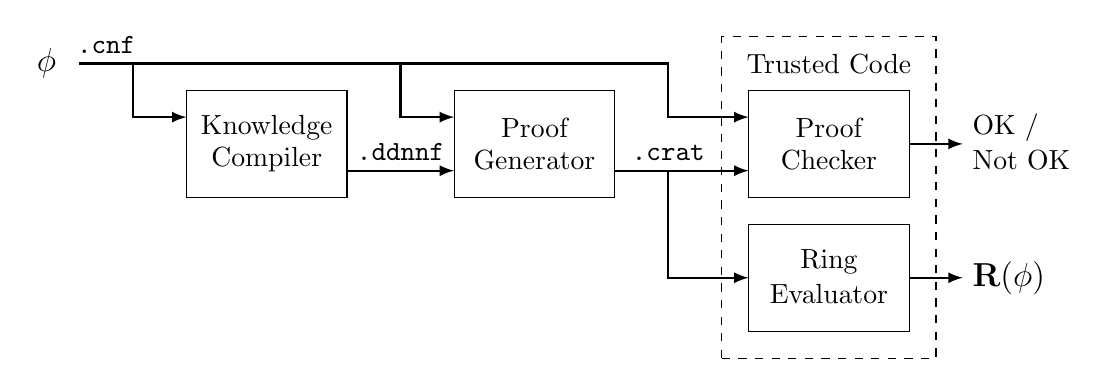
\begin{tikzpicture}[scale=0.17]
  \draw (8,10) rectangle (20,18);
  \node at (14,15.2) {Knowledge};
  \node at (14,12.8) {Compiler};

  \draw (28,10) rectangle (40,18);
  \node at (34,15.2) {Proof};
  \node at (34,12.8) {Generator};


  \draw (50,10) rectangle (62,18);
  \node at (56,15.2) {Proof};
  \node at (56,12.8) {Checker};

  \draw (50,0) rectangle (62,8);
  \node at (56,5.2) {Ring};
  \node at (56,2.8) {Evaluator};

  \draw[dashed] (48,-2) rectangle (64,22);
  \node at (56,20) {Trusted Code};

  %% CNF
  \draw[thick] (0,20) -- (44,20) -- (44,16) [-latex] -- (50,16);
  \draw[thick] (4,20) -- (4,16) [-latex] -- (8,16);
  \draw[thick] (24,20) -- (24,16) [-latex] -- (28,16);
  \node [left] at (-1,20) {\large {$\phi$}};
  \node [above] at (2,20) {\texttt{.cnf}};

  %% NNF
  \draw[thick] (20,12) [-latex] -- (28,12);
  \node [above] at (24,12) {\texttt{.ddnnf}};

  %% CRAT
  \draw[thick] (40,12) [-latex] -- (50,12);
  \draw[thick] (44,12) -- (44,4) [-latex] -- (50,4);
  \node [above] at (44,12) {\texttt{.crat}};

  %% OK/Not
  \draw[thick] (62,14) [-latex] -- (66,14) ;
  \node [right] at (66,15.2) { OK /} ;
  \node [right] at (66,12.8) { Not OK} ;
  \draw[thick] (62,4) [-latex] -- (66,4) ;
  \node [right] at (66,4) {\large {$\textbf{R}(\phi)$}};

\end{tikzpicture}
}
\caption{Certifying Tool Chain.
  The output of a standard knowledge compiler is converted into a combined graph/proof (CRAT) that can be independently checked and evaluated}
\label{fig:chain}
\end{figure}


Figure~\ref{fig:chain} illustrates the certifying knowledge compilation
and (weighted) model counting tool chain that we have developed.  A
{\em proof generator} generates a CRAT description from a d-DNNF
graph generated by \dfour{}, a state-of-the-art knowledge compiler.
A {\em proof checker} then verifies that the combination of CNF and CRAT files
satisfy our rules, and a {\em ring evaluator} can compute
either a standard or weighted model count from the POG\@ representation.
We evaluate the capabilities of this tool chain using
benchmark formulas from the 2022 standard and weighted model
competitions.  Our tools are able to handle all but the largest d-DNNF
graphs generated by \dfour{}.
As the dashed box in Figure~\ref{fig:chain} indicates, this tool chain
shifts the need for trustworthy code away from the complex and highly
optimized knowledge compiler to a relatively simple checker and
evaluator.  Importantly, the proof generator need not be
trustworthy---its errors will also be caught by the proof checker.

To further enhance the trustworthiness of our toolchain, we have
developed formally verified versions of the proof checker and ring
evaluator in the \lean{} proof assistant.  Running these two programs
has the effect of formally verifying both the logical equivalence of the POG to the input formula and the correctness of the count.
In addition, the
existence of a formally verified checker serves the important role of
establishing the soundness of our proof framework.

\section{Related Work}

Having a SAT solver generate a proof of unsatisfiability has a long
tradition~\cite{ZhangMalik} and has become widely accepted due to the
formulation of clausal proof systems for which proofs can readily be
generated and efficiently (and, in some cases, formally) checked
\cite{cruz-cade-2017,RAT,wetzler14_drattrim,Tan:2021}.  Some progress has also
been made on extending these proof systems to quantified Boolean
formulas~\cite{bryant:cade:2021,heule:JAR2014}.

Fichte, Hecher, and Roland~\cite{fichte:sat:2022} devised the MICE
proof framework for model counting programs.  Their proof rules are
based on the algorithmic steps commonly used by model counting
programs, and they present a series of lemmas and a theorem stating
that their checking framework is sound and complete.  They also
present experimental results for cases where they modify existing
model counters to also generate proof traces, and where they convert
d-DNNF graphs into a checkable form.  Our tool chain is not directly
comparable to theirs---they certify the output of a standard modeling
program, while we certify the output of a knowledge compiler and then
produce a certified standard or weighted model count.  There tool
chain can be applied to some programs that are pure model counters,
while ours can be applied to pure knowledge compilers.  Nonetheless,
we compare the performance of our tool chain to theirs as part of our
experimental evaluation in Section~\ref{sect:experimental}.  Our
experience with developing a formally verified CRAT proof checker has shown
us that, even for the well understood framework of extended
resolution, it can be challenging to formulate the full set of requirements to guarantee soundness.

We know of know other work addressing the more general question of
certifying the output of a knowledge compiler.


\section{Logical Foundations}

  Let $\varset$ denote a set of Boolean variables, and let $\assign$
  be an {\em assignment} of truth values to some subset of the
  variables, where $0$ denotes false and $1$ denotes true, i.e.,
  $\assign \colon \varset' \rightarrow \{0,1\}$ for some $\varset'
  \subseteq \varset$.  We say the assignment is {\em total} when it
  assigns a value to every variable ($\varset' = \varset$), and that
  it is {\em partial} otherwise.
  The set of all possible total assignments over
  $\varset$ is denoted $\uassign$.

For each variable $x \in \varset$,
  we define the {\em literals} $x$ and $\obar{x}$, where $\obar{x}$ is the
  negation of $x$. An
  assignment $\assign$ can be viewed as a set of literals, where
  we write $\lit \in \assign$ when $\lit = x$ and $\assign(x) = 1$ or when
  $\lit = \obar{x}$ and $\assign(x) = 0$.  We write the negation of literal $\lit$ as $\obar{\lit}$.  That is, $\obar{\lit} = \obar{x}$ when $\lit = x$ and
$\obar{\lit} = x$ when $\lit = \obar{x}$.


\begin{definition}[Boolean Formulas]
  The set of Boolean formulas is defined recursively.  Each
  formula $\phi$ has an associated {\em dependency set}
  $\dependencyset(\phi)  \subseteq \varset$, and a set of models $\modelset(\phi)$,
  consisting of total assignments that satisfy the formula:
  \begin{enumerate}
  \item Boolean constants $0$ and $1$ are Boolean formulas,
    with $\dependencyset(0) = \dependencyset(1) = \emptyset$, with $\modelset(0) = \emptyset$, and with $\modelset(1) = \uassign$.
  \item Variable $x$ is a Boolean formula, with $\dependencyset(x) = \{x\}$
    and $\modelset(x) = \{\assign \in \uassign | \assign(x)=1\}$.
  \item For formula $\phi$, its {\em negation}, written $\boolnot \phi$ is a Boolean formula,
    with $\dependencyset(\boolnot \phi) = \dependencyset(\phi)$ and $\modelset(\boolnot \phi) = \uassign - \modelset(\phi)$.
  \item For formulas $\phi_1, \phi_2, \ldots, \phi_k$, their {\em product} $\phi = \bigwedge_{i=1,k} \phi_i$ is a Boolean formula, with
      $\dependencyset(\phi) = \bigcup_{i=1,k} \dependencyset(\phi_i)$ and
      $\modelset(\phi) = \bigcap_{i=1,k} \modelset(\phi_i)$.
  \item For formulas $\phi_1, \phi_2, \ldots, \phi_k$, their {\em sum} $\phi = \bigvee_{i=1,k} \phi_i$ is a Boolean formula, with
      $\dependencyset(\phi) = \bigcup_{i=1,k} \dependencyset(\phi_i)$ and
      $\modelset(\phi) = \bigcup_{i=1,k} \modelset(\phi_i)$.
  \end{enumerate}
\label{def:boolean}
\end{definition}


  We highlight two special classes of Boolean formulas.  A formula is
  in {\em negation normal form} when negation is applied only to variables.  A
  formula is in {\em conjunctive normal form} (CNF) when 1) it is in
  negation normal form, and 2) sum is applied only to literals.  A CNF
  formula can be represented as a set of {\em clauses}, each of which is a
  set of literals.  Each clause represents the sum of the
  literals, and the formula is the product of its clauses.  We use
  set notation to reference the clauses in a formula and the
  literals in a clause.  A clause consisting of a single literal is referred to as a {\em unit} clause.
This literal must be assigned value $1$ by any satisfying assignment of the formula.

  A {\em partitioned-operation formula}
 satisfies the following for all product and sum operations:
      \begin{itemize}
      \item The arguments to a product must have disjoint dependency sets.  That is, operation
        $\bigwedge_{i=1,k} \phi_i$ requires $\dependencyset(\phi_i) \cap \dependencyset(\phi_j) = \emptyset$ for $1 \leq i < j \leq k$.
      \item The arguments to a sum must have disjoint models.  That is, operation
        $\bigvee_{i=1,k} \phi_i$ requires $\modelset(\phi_i) \cap \modelset(\phi_j) = \emptyset$ for $1 \leq i < j \leq k$.
      \end{itemize}
     We let $\pand$ and $\por$ denote the product and sum operations in a partitioned-operation formula.

  \section{Ring Evaluation of a Boolean Formula}

We propose a general framework for summarizing properties of Boolean
formulas inspired by the formulation of {\em algebraic model counting}
by Kimmig, et al.~\cite{kimmig:jal:2017}.

\begin{definition}[Commutative Ring]
  A {\em commutative ring} $\ring$ is an algebraic structure
  $\langle \dset, \radd, \rmul, \addident, \mulident \rangle$,
  with elements in the set $\dset$ and with commutative and
  associative operations $\radd$ (addition) and $\rmul$ (multiplication),
  such that multiplication distributes
  over addition.  $\addident$ is the additive identity and $\mulident$ is
  the multiplicative identity.  Every element $a \in \dset$ has an
  {\em additive inverse} $-a$ such that $a + -a = \addident$.
\label{def:ring}
\end{definition}
We write $a - b$ as a shorthand for $a + -b$.

\begin{definition}[Ring Evaluation Problem]
\label{def:ring_evaluation}
  For commutative ring $\ring$, a {\em ring labeling} associates a value $w(x) \in \dset$ with
  every variable $x \in \varset$.  We then define $w(\obar{x})$ to equal $\mulident-w(x)$.

  For Boolean formula $\phi$, and ring labeling $w$, the {\em ring evaluation problem} is to compute:
  \begin{eqnarray}
    \rep(\phi, w) & = & \sum_{\alpha \in \modelset(\phi)} \;\; \prod_{\lit \in \alpha} w(\ell) \label{eqn:rep}
  \end{eqnarray}
  In this equation, sum $\sum$ is computed using addition operation $\radd$, and product $\prod$ is computed using multiplication operation $\rmul$.
\label{def:labeling}
\end{definition}

Many important properties of Boolean formulas can be
expressed as ring evaluation problems.  The
{\em model counting} problem for formula $\phi$ requires determining $|\modelset(\phi)|$.
It can be cast as a ring evaluation problem by having $\radd$ and
$\rmul$ be addition and multiplication over rational numbers and using
label $w(x) = 1/2$ for every variable $x$.
Ring evaluation of formula $\phi$ will then compute the {\em density} of
the formula, i.e., the fraction of all possible total assignments that are
models.  For $n = |\varset|$, scaling the density by $2^n$ will then
yield the number of models.

The {\em weighted model counting} (WMC) problem is also defined over
rational numbers.  Some formulations of WMC allow
independently assigning weights $W(x)$ and $W(\obar{x})$ for each variable $x$ and its complement, with the possibility that
$W(x) + W(\obar{x}) \not = 1$.
We can convert this more general form into a
ring evaluation problem by letting $r(x) = W(x) + W(\obar{x})$,
performing ring evaluation with label $w(x) = W(x)/r(x)$ for each
variable $x$, and then computing the final result as $\rep(\phi, w)\;
\rmul\; \prod_{x \in \varset} r(x)$.  Of course, this requires that $r(x) \not = 0$ for all $x \in \varset$.

The {\em function hashing problem} provides a test
of inequivalence for Boolean formulas.  That is, for $n = |\varset|$, let $\ring$ be a
finite  field with $|\dset| = m$ such that $m \geq 2 n$.  For each $x \in \varset$, chose a value from $\dset$ at random for $w(x)$.  Two formulas
$\phi_1$ and $\phi_2$ will clearly have $\rep(\phi_1, w) = \rep(\phi_2, w)$
if they are logically equivalent.  If they are not equivalent, then
the probability that $\rep(\phi_1, w) \not = \rep(\phi_2, w)$ will be at
least $\left(1-\frac{1}{m}\right)^n \geq \left(1-\frac{1}{2n}\right)^n > 1/2$.
Therefore, ring evaluation can be used as part of a
randomized algorithm for equivalence testing~\cite{blum:ipl:1980}.

We compare ring evaluation to algebraic model counting in Section~\ref{sect:future}.

\section{Partitioned-Operation Graphs (POGs)}

Performing ring evaluation on an arbitrary Boolean formula could be intractable, but it is straightforward for a formula with partitioned operations:
\begin{proposition}
<<<<<<< Updated upstream
For any labeling $w$, ring evaluation with operations $\boolnot$, $\pand$, and $\por$ satisfies:
=======
\label{prop:ring:eval}
Ring evaluation with operations $\boolnot$, $\pand$, and $\por$ satisfies the following for any labeling $w$:
>>>>>>> Stashed changes
\begin{eqnarray}
%% V1
\textstyle
\rep(\boolnot \phi,\; w) &=& \mulident - \rep(\phi, w) \label{eqn:ring:negation} \\
\textstyle
\rep\left(\Pand_{i=1,k} \phi_i,\; w \right) &=& \prod_{i=1,k} \rep(\phi_i, w) \label{eqn:ring:product} \\
\textstyle
\rep\left(\Por_{i=1,k} \phi_i,\; w\right) &=& \sum_{i=1,k} \rep(\phi_i, w) \label{eqn:ring:sum}
%% V2
%\rep(\boolnot \phi, w) &=& \mulident - \rep(\phi, w) \label{eqn:ring:negation} \\
%\rep\left(\phi_1, w \pand \dots \pand \phi_k, w \right) &=& \prod_{i=1..k} \rep(\phi_i, w) \label{eqn:ring:product} \\
%\rep\left(\phi_1, w \por \dots \por \phi_k, w \right) &=& \sum_{i=1..k} \rep(\phi_i, w) \label{eqn:ring:sum}
%\rep\left(\Pand_{i=1,k} \phi_i, w \right) &=& \prod_{i=1,k} \rep(\phi_i, w) \label{eqn:ring:product} \\
%\rep\left(\Por_{i=1,k} \phi_i, w\right) &=& \sum_{i=1,k} \rep(\phi_i, w) \label{eqn:ring:sum}
\end{eqnarray}
\end{proposition}

A {\em partitioned-operation graph} (POG) is a directed, acyclic graph
with nodes $N$ and edges $E \subseteq N \times N$.  We denote nodes with boldface symbols, such as $\nodeu$ and $\nodev$.
When $(\nodeu,\nodev) \in E$,
node $\nodev$ is said to be a {\em child} of node $\nodeu$.
The in- and out-degrees of node $\nodeu$ are defined as $\indegree(\nodeu) = | E \cap (N \times \{\nodeu\}) |$, and
$\outdegree(\nodeu) = | E \cap (\{\nodeu\} \times N) |$.
Node $\nodeu$ is said to be {\em terminal} if $\outdegree(\nodeu) = 0$.  A terminal node is labeled by a Boolean constant or variable.
Node $\nodeu$ is said to be {\em nonterminal} if $\outdegree(\nodeu) > 0$.
A nonterminal node is labeled by one of the three Boolean operations: $\boolnot$, $\pand$ or $\por$.
Node $\nodeu$ can be labeled with $\boolnot$ only if $\outdegree(\nodeu) = 1$.
It can be labeled with operation $\pand$ or $\por$ only if it satisfies the partitioning restriction for that operation.
There is a unique {\em root node} $\noder$ such that $\indegree(\noder) = 0$.
As can be seen, a POG is simply a way to represent a partitioned-operation
formula with a sharing of common subformulas.  Indeed, every node the graph can be viewed as a partitioned-operation formula, and so we write
$\phi_{\nodeu}$ as the formula denoted by node $\nodeu$.
Each such formula has a set of models, and we write $\modelset(\nodeu)$ as a shorthand for $\modelset(\phi_{\nodeu})$.

We define the {\em size} of POG $P$, written $|P|$ to be the
the number of nodes labeled $\pand$ or $\por$ plus the number of edges from these nodes to their children.  Ring
evaluation of $P$ can be performed with at most $|P|$ ring
operations by traversing the graph from the terminal nodes up to
the root, computing a value $\rep(\nodeu, w)$ for each node $\nodeu$.
The final result is then $\rep(\noder, w)$.

POGs are inspired by the d-DNNF graphs devised by Darwiche for
representing Boolean functions \cite{darwiche:jair:2002}.
POGs generalize d-DNNF in two ways:
\begin{itemize}
\item They allow negation of arbitrary nodes in the graph, not just
  variables.  As we have seen, ring evaluation can readily handle negation, and so we allow it in the interest of generality.
%%  Negation could be useful in some contexts, such as when
%%  converting binary decision diagrams (BDDs) having complemented
%%  edges~\cite{brace-dac-1990,minato-dac-1990} into POGs.

\item They allow arbitrary arguments to a $\por$ operation, as long as
  they have disjoint models.  By contrast, each
  sum node $\nodeu$ in a d-DNNF can have two children $\nodeu_1$ and $\nodeu_0$, and for these there must be a {\em decision variable} $x$ such that
  any total assignment $\assign \in  \modelset(\nodeu_b)$ has $\assign(x)=b$, for $b \in \{0,1\}$.
Our generalization is provided to allow an
  encoding of Sentential Decision Diagrams (SDDs)~\cite{darwiche:ijcai:2011} as
  POGs.  This is discussed in Section~\ref{sect:future}, describing possible future research.
\end{itemize}
  Both of these generalizations allow more flexibility in the POG
  representation while maintaining the ability to efficiently perform ring evaluation.

\section{Clausal Proof Frameworks}

A proof in our framework takes the form of a sequence of clause addition
and deletion steps, with each step maintaining logical equivalence to
the original formula.  More precisely, the status of the proof at any step will be represented by
a set of {\em active} clauses $\phi$, i.e., those that
have been added but not yet deleted.  Our framework is based
on {\em extended} resolution~\cite{Tseitin:1983}, meaning that proof
steps can introduce new {\em extension variables}.  Let $Z$
denote the set of extension variables occuring in formula $\phi$.
Starting with input formula $\inputformula$,
we want to maintain the invariant that
$\inputformula \ifandonlyif \exists Z\,\phi$.

Clauses can be added in two different ways.  One is when they serve as
the {\em defining clauses} for an extension variable.  We will use
this form only when defining $\pand$ and $\por$ operations, as is
described in Section~\ref{sect:crat}.  The other is by {\em
  implication redundancy}.  That is, we can add clause $C$ to the set
of clauses forming formula $\phi$ when $\phi \imply C$.  Clauses can
also be deleted through implication redundancy.  That is, given a set
of clauses $\{C\} \cup \phi$, we can remove $C$ if $\phi \imply C$.

We use {\em reverse unit propagation} (RUP) to certify
implication redundancy when adding or deleting
clauses~\cite{goldberg,vangelder08_verifying_rup_proofs}.
RUP
is the core rule supported by standard
proof checkers~\cite{RAT,wetzler14_drattrim} for propositional logic.
It is a way to check a sequence of applications of the resolution proof rule~\cite{robinson-1965}.
Let $C = \lit_1 \lor \lit_2 \lor \cdots \lor \lit_p$ be a clause to be
proved redundant with respect to formula $\phi$.  Let $D_1, D_2, \ldots, D_k$ be a sequence of supporting
{\em antecedent} clauses, such that each $D_i$ is in $\phi$.
A RUP step
proves that $\bigwedge_{1\leq i \leq k} D_i \imply C$ by showing
that the combination of the antecedents plus the negation of $C$ leads
to a contradiction.  The negation of $C$ is the formula
$\overline{\lit}_1 \land \overline{\lit}_2 \land \cdots \land
\overline{\lit}_p$ having a CNF representation consisting of $p$ unit
clauses of the form $\obar{\lit}_i$ for $1 \leq i \leq p$.  A RUP
check processes the clauses of the antecedent in sequence, inferring
additional unit clauses.  In processing clause $D_i$, if all but one
of the literals in the clause is the negation of one of the
accumulated unit clauses, then we can add this literal to the
accumulated set.  That is, all but this literal have been falsified,
and so it must be set to true for the clause to be satisfied.  The
final step with clause $D_k$ must cause a contradiction, i.e., all of
its literals are falsified by the accumulated unit clauses.

Compared to the proofs of unsatisfiability generated by SAT solvers,
it can be seen that ours has important differences.  Most
significantly, we want our proofs to maintain logical equivalence at
each step, whereas an unsatisfiability proof need only guarantee that
no proof step makes a satisfiable set of clauses become
unsatisfiable.  Therefore, our proofs must justify clause deletions as well as clause additions.


\section{The CRAT POG Representation and Proof System}
\label{sect:crat}


A CRAT file provides both a declaration of a POG, as well as an easily checkable
proof that a Boolean formula, given in conjunctive normal
form, is logically equivalent to the POG, thus enabling certified
knowledge compilation.
%% The proof system is based on extended
%% resolution~\cite{Tseitin:1983} with reverse unit propagation
%% (RUP)~\cite{goldberg,vangelder08_verifying_rup_proofs} as the core method for
%% proving that a set of clauses logically implies another clause.
%% Alternate version
%% knowledge compilation.  The proof system is based on extended
%% resolution~\cite{Tseitin:1983} with reverse unit propagation
%% (RUP)~\cite{goldberg,vangelder08_verifying_rup_proofs} as the core method for
%% proving that a set of clauses logically implies another clause.
%%
%% As an example, consider the formula $\varphi = (\obar{a} \lor b) \land (\obar{b} \lor c \lor \obar{e}) \land (\obar c \lor d)$
%% and a RUP step to derive the target clause $(\obar{a} \lor d \lor \obar{e})$ from the three clauses from $\varphi$.
%% A RUP proof would take the following form.  We start with the assignment that falsifies the target clause. This assignment
%% is extended by clauses in $\varphi$ that become unit and eventually the empty clause. In the illustration below, the
%% involved clauses (antecedents) are shown in the order that they became unit / falsified.
%%
%% \begin{center}
%%   \begin{tabular}{lcccc}
%%          & \makebox[15mm]{Target}    & \makebox[10mm]{} & \makebox[10mm]{Antecedents} & \makebox[10mm]{} \\
%%   Clause & $\obar{a} \lor d \lor \obar{e}$ & $\obar{c} \lor d$  & $\obar{e} \lor \obar{b} \lor c$   & $\obar{a} \lor b$ \\
%%   \midrule
%%   Units  & $a$, $\obar{d}$, $e$      &  $\obar{c}$             & $\obar{b}$                         & $\nil$ \\
%%   \end{tabular}
%% \end{center}
%%
%% RUP is an alternative formulation of resolution.  For target clause
%% $C$, it can be seen that applying resolution operations to the
%% antecedent clauses from right to left will derive a clause $C'$ such
%% that $C' \subseteq C$.  By {\em subsumption} %~\cite{philipp:lpar:2017},
%% we then have $C' \rightarrow C$.  Compared to listing each resolution
%% operation as a separate step, using RUP as the basic proof step makes
%% the proofs more compact.
%%
%% As is shown in Figure~\ref{fig:chain}
%% two programs are involved in producing a certified compilation of a formula:
%% \begin{itemize}
%% \item The {\em proof generator} produces a CRAT file that both defines the POG and gives a proof that the POG is logically equivalent to the input formula.
%% As the figure indicates, the generator starts with the output of another knowledge compiler, such as one generating a d-DNNF representation of the formula.
%% \item The {\em proof checker} ensures that all of the proof conditions are satisfied.
%% \end{itemize}
%% >>>>>>> 9c1793da858d00e5d4022d6d33c009848ba2083b

The CRAT format draws its inspiration from the LRAT format for Boolean
formulas~\cite{lrat} and the QRAT format for quantified Boolean
formulas (QBF)~\cite{heule:JAR2014}.  The following are its key properties:
\begin{itemize}
  \item
  The file contains declarations of $\pand$ and $\por$ operations to describe the POG.
  Declaring a node $\nodeu$
implicitly adds an {\em extension} variable $u$ and a set of {\em defining} clauses
  encoding the product or sum operation.
  This is the only means for adding extension variables to the proof.
\item Boolean negation is supported implicitly by allowing the
  arguments of the $\por$ and $\pand$ operations to be literals and not just
  variables.
\item
  The file contains explicit clause addition steps.
  A clause can only be added if it is logically implied by the existing clauses.
  A sequence of clause identifiers must be listed as {\em hints} providing a RUP verification of the implication.
\item
  The file contains explicit clause deletion steps.
  A clause can only be deleted if it is logically implied by the remaining clauses.
  A sequence of clause identifiers must be listed as {\em hints} providing a RUP verification of the implication.
\item The checker must track the dependency set for every input and
  extension variable.  For each $\pand$ operation, the checker must ensure that the dependency sets for its arguments are disjoint.
  The associated extension variable has a dependency set equal to the union of those of its arguments.
\item Declaring a $\por$ operation requires a sequence of clauses
  providing a RUP proof that the arguments are mutually exclusive.
  Only binary $\por$ operations are allowed.  Generalizing to $k$ arguments would require
  $k\,(k-1)/2$ proofs of disjointness.
\end{itemize}

\subsection{Syntax}
\label{subsection:syntax}

\begin{table}
  \caption{CRAT Step Types.  $C$: clause identifier, $L$: literal, $V$: variable}
  \label{tab:crat:syntax}
\centering{
  \begin{tabular}{lllll}
    \toprule
    \multicolumn{4}{c}{Rule} & \multicolumn{1}{c}{Description} \\
    \midrule
    \makebox[5mm][l]{$C$} & \makebox[10mm][l]{\tt a}  & \makebox[15mm][l]{$L^{*}$ {\tt 0}} & \makebox[15mm][l]{$C^{+}$ {\tt 0}}  & \makebox[20mm][l]{Add RUP clause} \\
     & {\tt d} & $C$             & $C^{+}$  {\tt 0} & Delete RUP clause \\
    \midrule
    $C$    & {\tt p} & $V \; L^{*}$ {\tt 0}    &                  & Declare $\pand$ operation \\
    $C$    & {\tt s} & $V \; L \; L$    & $C^{+}$ {\tt 0}  & Declare $\por$ operation \\
    \midrule
     & {\tt r} & $L$             &            & Declare root literal\\
    \bottomrule
  \end{tabular}
  }
\end{table}

Table~\ref{tab:crat:syntax} shows the declarations that can occur in a CRAT file.
The checker is provided with the input formula as a separate file.
As with other clausal proof formats, a variable is
represented by a positive integer $v$, with the first ones being input
variables and successive ones being extension variables.  Literal $\lit$
is represented by a signed integer, with $-v$ being the logical negation of
variable $v$.  Each clause is indicated by a positive integer
identifier $C$, with the first ones being the IDs of the input clauses and successive
ones being the IDs of added clauses.  Clause identifiers must be totally ordered,
such that any clause identifier $C'$ given in the hints when adding clause $C$ must have $C' < C$.

The first set of proof rules are similar to those in other clausal
proofs.
Clauses can be added via RUP addition
(command {\tt a}), with a sequence of antecedent clauses (the
``hints'').
Similarly for clause deletion (command {\tt d}).

\begin{table}
\caption{Defining Clauses for Product (A) and Sum (B) Operations}
\begin{minipage}{0.54\textwidth}
\begin{center}
\begin{tabular}{cccccc}
\multicolumn{6}{c}{(A).  Product Operation $\pand$}\\
\toprule
\makebox[10mm]{ID} & \multicolumn{5}{c}{Clause} \\
\midrule
  $i$ & $v$ & $-\lit_1$ & $-\lit_2$ & $\cdots$ & $-\lit_k$\\
  $i\!+\!1$ & $-v$ & $\lit_1$  \\
  $i\!+\!2$ & $-v$ & $\lit_2$  \\
  & $\ldots$ \\
  $i\!+\!k$ & $-v$ & $\lit_k$  \\
\bottomrule
\end{tabular}
\end{center}
\end{minipage}
\begin{minipage}{0.44\textwidth}
\begin{center}
\begin{tabular}{cccc}
\multicolumn{4}{c}{(B).  Sum Operation $\por$}\\
\toprule
\makebox[10mm]{ID} & \multicolumn{3}{c}{Clause} \\
\midrule
  $i$ & $-v$ & $\lit_1$ & $\lit_2$ \\
  $i\!+\!1$ & $v$ & $-\lit_1$ \\
  $i\!+\!2$ & $v$ & $-\lit_2$ \\
\bottomrule
$\;$ \\
$\;$ \\
\end{tabular}
\end{center}
\end{minipage}
\label{tab:defining}
\end{table}

The declaration of a {\em product} operation, creating a node with operation $\pand$,
 has the form:
\begin{center}
\begin{tabular}{ccccccccc}
  \makebox[5mm]{$i$} & \makebox[5mm]{{\tt p}} & \makebox[5mm]{$v$} & \makebox[5mm]{$\lit_1$} & \makebox[5mm]{$\lit_2$} &
  \makebox[5mm]{$\cdots$} & \makebox[5mm]{$\lit_k$} & \makebox[5mm]{\tt 0} \\
\end{tabular}
\end{center}
Integer $i$ is a new clause ID, $v$ is a positive integer that does not
correspond to any previous variable, and $\lit_1, \lit_2, \ldots, \lit_k$ is a sequence of $k$
integers representing literals of existing variables.
As Table~\ref{tab:defining}(A) shows,
this declaration implicitly causes $k+1$ clauses to be added to the proof, defining extension variable $v$ to be the product of its arguments.

The dependency sets for the arguments represented by each pair of
literals $\lit_i$
and $\lit_{j}$ must
be disjoint, for $1 \leq i < j \leq k$.  A product operation may have no arguments,
representing Boolean constant $1$.  The only clause added to the proof will be
the unit literal $v$.  A reference to literal $-v$ then becomes a way
of representing constant $0$.

The declaration of a {\em sum} operation, creating a node with operation $\por$, has the form:
\begin{center}
\begin{tabular}{ccccccc}
  \makebox[5mm]{$i$} & \makebox[5mm]{{\tt s}} & \makebox[5mm]{$v$} & \makebox[5mm]{$\lit_1$} & \makebox[5mm]{$\lit_2$}
\makebox[5mm]{$H$} & \makebox[5mm]{$\texttt{0}$} \\
\end{tabular}
\end{center}
Integer $i$ is a new clause ID, $v$ is a positive integer that does
not correspond to any previous variable, and $\lit_1$ and $\lit_2$ are
signed integers representing literals of existing variables.  Hint $H$
consists of a
sequence of clause IDs, all of which must be defining clauses for other POG operations.
As Table~\ref{tab:defining}(B) shows,
this declaration implicitly causes three clauses to be added to the proof, defining extension variable $v$ to be the sum of its arguments.
The hints must provide a RUP proof of the clause $\obar{\lit}_1 \lor \obar{\lit}_2$, showing that the two children of this node have disjoint models.

Finally, the literal denoting the root of the POG is declared with the
{\tt r} command.  It can occur anywhere in the file.  Typically, it
will be the extension variable representing the root of a graph, but in
degenerate cases it can be the positive or negative literal of an
input variable.

\subsection{Semantics}

The defining clauses for a product or sum
operation uniquely define the value of its extension variable for any assignment of values to the argument variables.
For the
extension variable $u$ associated with any POG node $\nodeu$, we can therefore
assume that any total assignment $\assign$ to the input variables will
also assign a value to $u$ such that $\assign(u) =
1$ if and only if $\assign \in \modelset(\nodeu)$.  For a POG with
root literal $r$, we can define its set of models $\modelset(P)$ as
the set of all total assignments $\assign$ such that $\assign(r) = 1$.

%% A CRAT proof follows the same general form as a QRAT dual
%% proof~\cite{bryant:cade:2021}---one that ensures that each clause
%% addition and each clause deletion preserves equivalence.  With CRAT,
%% however, clauses are defined both explicitly and implicitly.  Starting
%% with the set of input clauses, the proof consists of a sequence of
%% steps that both add and delete clauses.  Each addition must be truth
%% preserving, that is, any satisfying total assignment for the set of clauses
%% before clause addition should still be a satisfying assignment afterwards.
%% Each deletion must be falsehood preserving.  That is, there can be no
%% new satisfying assignments when the clause is deleted.

The sequence of operator declarations, asserted clauses, and
clause deletions represents a systematic transformation of the input formula
into a POG\@.  Validating all of these steps serves to prove that the
POG is logically equivalent to the input formula.
At the completion of the proof, the following conditions must hold:
\begin{itemize}
\item There should exactly one remaining clause that was added via RUP
  addition, and this should be a unit clause consisting of the root literal $r$.
\item All of the input clauses have been deleted.
\end{itemize}
The sequence of clause addition steps provide a {\em forward implication} proof that
$\modelset(\phi) \subseteq \modelset(P)$.  That is, any total
assignment $\assign$ satisfying the input formula must also satisfy
the formula represented by the POG\@.
Conversely,
each proof step that deletes an input clause proves that any
total assignment $\alpha$ that falsifies the clause must
assign $\assign(r) = 0$.  Deleting all but the final asserted clause and all input clauses provides a {\em reverse implication} proof
that
$\modelset(P) \subseteq \modelset(\phi)$.

\subsection{CRAT Example}

\begin{figure}
\begin{minipage}{0.62\textwidth}
(A)  Input Formula\\[1.2ex]
\begin{tabular}{lll}
\toprule
\makebox[5mm]{ID} & \makebox[15mm]{Clauses} & \\
\midrule
1 & \texttt{-1 3 -4} & \texttt{0} \\
2 & \texttt{-1 -3 4} & \texttt{0} \\
3 & \texttt{3 -4} & \texttt{0}\\
4 & \texttt{1 -3 4} & \texttt{0} \\
5 & \texttt{-1 -2} & \texttt{0} \\
\bottomrule
\end{tabular}
\\[1.8ex]
(C) POG Declaration\\[1.2ex]
\begin{tabular}{llll}
\toprule
\makebox[5mm]{ID} & \multicolumn{2}{l}{CRAT line} & Explanation \\
\midrule
6 & \texttt{p 5 -3 -4} & \texttt{0} & $p_5 = \obar{x}_3 \pand \obar{x}_4$ \\
9 & \texttt{p 6 3 4} & \texttt{0} & $p_6 = x_3 \pand x_4$ \\
12 & \texttt{s 7 5 6 7 10} & \texttt{0} & $s_7 = p_5 \por p_6$ \\
15 & \texttt{p 8 -1 7} & \texttt{0} & $p_8 = \obar{x}_1 \pand s_7$ \\
18 & \texttt{p 9 1 -2 7} & \texttt{0} & $p_9 = x_1 \pand \obar{x}_2 \pand s_7$ \\
22 & \texttt{s 10 8 9 16 19} & \texttt{0} & $s_{10} = p_8 \por p_9$ \\
 & \texttt{r 10} && Root $r = s_{10}$\\
\bottomrule
\end{tabular}
\end{minipage}
\begin{minipage}{0.35\textwidth}
(B) POG Representation \\
\input{dd/eg4}
\end{minipage}
%% Break
\\[2.5ex]
\begin{minipage}{0.45\textwidth}
(D) Implicit Clauses\\[1.2ex]
\begin{tabular}{llll}
\toprule
\makebox[5mm]{ID} & \multicolumn{2}{l}{Clauses} & Explanation \\
\midrule
\texttt{6} & \texttt{5 3 4} & \texttt{0} & Define $p_5$ \\
\texttt{7} & \texttt{-5 -3} & \texttt{0} & \\
\texttt{8} & \texttt{-5 -4} & \texttt{0} & \\
\midrule
\texttt{9} & \texttt{6 -3 -4} & \texttt{0} & Define $p_6$ \\
\texttt{10} & \texttt{-6 3} & \texttt{0} & \\
\texttt{11} & \texttt{-6 4} & \texttt{0} & \\
\midrule
\texttt{12} & \texttt{-7 5 6} & \texttt{0} & Define $s_7$ \\
\texttt{13} & \texttt{7 -5} & \texttt{0} & \\
\texttt{14} & \texttt{7 -6} & \texttt{0} & \\
\midrule
\texttt{15} & \texttt{8 1 -7} & \texttt{0} & Define $p_8$ \\
\texttt{16} & \texttt{-8 -1} & \texttt{0} & \\
\texttt{17} & \texttt{-8 7} & \texttt{0} & \\
\midrule
\texttt{18} & \texttt{9 -1 2 -7} & \texttt{0} & Define $p_9$ \\
\texttt{19} & \texttt{-9 1} & \texttt{0} & \\
\texttt{20} & \texttt{-9 -2} & \texttt{0} & \\
\texttt{21} & \texttt{-9 7} & \texttt{0} & \\
\midrule
\texttt{22} & \texttt{-10 8 9} & \texttt{0} & Define $s_{10}$ \\
\texttt{23} & \texttt{10 -8} & \texttt{0} & \\
\texttt{24} & \texttt{10 -9} & \texttt{0} & \\
\bottomrule
\end{tabular}
\end{minipage}
\begin{minipage}{0.49\textwidth}
(E) CRAT Assertions\\[1.2ex]
\begin{tabular}{llllll}
\toprule
\makebox[5mm]{ID} & \multicolumn{2}{l}{Clause} & \multicolumn{2}{l}{Hints} & Explanation \\
\midrule
\texttt{25} & \texttt{a 5 1 3} & \texttt{0} & \texttt{3 6} & \texttt{0} & $\obar{x}_1 \land \obar{x}_3 \imply p_5$ \\
\texttt{26} & \texttt{a 6 1 -3} & \texttt{0} & \texttt{4 9} & \texttt{0} & $\obar{x}_1 \land x_3 \imply p_6$ \\
\texttt{27} & \texttt{a 3 7 1} & \texttt{0} & \texttt{13 25} & \texttt{0} & $\obar{x}_3 \land \obar{x}_1 \imply s_7$  \\
\texttt{28} & \texttt{a 7 1} & \texttt{0} & \texttt{27 14 26} & \texttt{0} & $\obar{x}_1 \imply s_7$  \\
\texttt{29} & \texttt{a 8 1} & \texttt{0} & \texttt{28 15} & \texttt{0} & $\obar{x}_1 \imply p_8$  \\
\texttt{30} & \texttt{a 5 -1 3} & \texttt{0} & \texttt{1 6} & \texttt{0} & $x_1 \land \obar{x}_3 \imply p_5$ \\
\texttt{31} & \texttt{a 6 -1 -3} & \texttt{0} & \texttt{2 9} & \texttt{0} & $x_1 \land x_3 \imply p_6$ \\
\texttt{32} & \texttt{a 3 7 -1} & \texttt{0} & \texttt{13 30} & \texttt{0} & $\obar{x}_3 \land x_1 \imply s_7$  \\
\texttt{33} & \texttt{a 7 -1} & \texttt{0} & \texttt{32 14 31} & \texttt{0} & $x_1 \imply s_7$  \\
\texttt{34} & \texttt{a 9 -1} & \texttt{0} & \texttt{5 33 18} & \texttt{0} & $x_1 \imply p_9$  \\
\texttt{35} & \texttt{a 1 10} & \texttt{0} & \texttt{23 29} & \texttt{0} & $\obar{x}_1 \imply s_{10}$  \\
\texttt{36} & \texttt{a 10} & \texttt{0} & \texttt{35 24 34} & \texttt{0} & $s_{10}$ \\
\bottomrule
\end{tabular}
\\[1.5ex]
(F) Input Clause Deletions\\[1.2ex]
\begin{tabular}{lllll}
  \toprule
 \multicolumn{3}{l}{CRAT line} & Explanation\\
\midrule
 \texttt{d 1} & \texttt{36 8 10 12 16 21 22} & \texttt{0} & Delete clause 1 \\
 \texttt{d 2} & \texttt{36 7 11 12 16 21 22} & \texttt{0} & Delete clause 2 \\
 \texttt{d 3} & \texttt{36 8 10 12 17 19 22} & \texttt{0} & Delete clause 3 \\
 \texttt{d 4} & \texttt{36 7 11 12 17 19 22} & \texttt{0} & Delete clause 4 \\
 \texttt{d 5} & \texttt{36 16 20 22} & \texttt{0} &  Delete clause 5 \\
\bottomrule
\end{tabular}
\end{minipage}
\caption{Example formula (A), its POG representation (B), and its CRAT proof (C), (E), and (F)}
\label{fig:eg4:all}
\end{figure}

Figure \ref{fig:eg4:all} illustrates an example formula and shows how
the CRAT file declares its POG representation.  The input formula (A)
consists of five clauses over variables $x_1$, $x_2$, $x_3$, and
$x_4$.  The generated POG (B) has six nonterminal nodes representing
four products and two sums.  We name these by the node
type (product $\nodep$ or sum $\nodes$), subscripted by the ID of the
extension variable.
% We denote the extension variable for nodes $\nodep_i$ and $\nodes_j$ as $p_i$ and $s_j$, respectively.
  The first part of the CRAT file (C) declares
these nodes using clause IDs that increment by three or four,
depending on whether the node has two children or three.  The last two
nonzero values in the sum declarations are hints providing the
required mutual exclusion proof.

We step through a detailed example to provide a better understanding of the CRAT proof framework.
Figure
\ref{fig:eg4:all}(D) shows the defining clauses that are implicitly
defined by the POG operation declarations.  These do not appear in the
CRAT file.  Referring back to the declarations of the sum nodes in
Figure \ref{fig:eg4:all}(C), we can see that the declaration of node
$\nodes_7$ had clause IDs 7 and 10 as hints.  We can see in Figure
\ref{fig:eg4:all}(A) that these two clauses resolve to the clause
$\obar{p}_5 \lor \obar{p}_6$, showing that the two children of $\nodes_7$
have disjoint models.  Similarly, node $\nodes_{10}$ is declared as having
clause IDs 16 and 19 as hints.  These resolve to the clause
$\obar{p}_8 \lor \obar{p}_9$, showing that the two children of
$\nodes_{10}$ have disjoint models.

Figure \ref{fig:eg4:all}(E) provides the sequence of assertions
leading to unit clause 36, consisting of the literal $s_{10}$.  This clause indicates that $\nodes_{10}$ is implied by the input clauses, i.e.,
any total assignment $\assign$
satisfying the input clauses must have $\assign(s_{10}) = 1$.
Working backward, we can see that
clause 29 indicates that variable $p_8$ will be implied by the input
clauses when $\assign(x_1) = 0$, while clause 34 indicates that node $p_9$ will
be implied by the input clauses when $\assign(x_1) = 1$.  These serve as the
hints for clause 36.

Figure \ref{fig:eg4:all}(F) shows the RUP proof steps required to
delete the input clauses.  Consider the first of these, deleting
input clause $\obar{x}_1 \lor x_3 \lor \obar{x}_4$.  The requirement is to show
that there is no total assignment $\assign$ that falsifies this clause but assigns $\assign(s_{10}) = 1$.
The proof proceeds by first assuming that the clause is false, requiring
$\assign(x_1) = 1$, $\assign(x_3) = 0$, and $\assign(x_4) = 1$.  The hints then consist of unit
clauses (e.g., clause 36 asserting that $\alpha(p_{10}) = 1$) or
clauses that cause unit propagation.  Hint clauses 8 and 10 force the
assignments $\assign(p_5) = \assign(p_6) = 0$.  These, plus hint clause 12 force
$\assign(s_7) = 0$.  This, plus hint clauses 16 and 21 force $\assign(p_8) = \assign(p_9) = 0$, leading
via clause 22 to $\assign(s_{10}) = 0$.  But this contradicts clause 36,
completing the RUP proof.  The deletion hints for the other input
clauses follow similar patterns---they work from the bottom nodes of
the POG upward, showing that any total assignment that falsifies the clause
must assign $\assign(s_{10}) = 0$.

Deleting the asserted clauses is so simple that we do not show it.  It
involves simply deleting the clauses from clause number 35 down to
clause number 25, with each deletion using the same hints as were used
to add that clause.  In the end, therefore, only the defining clauses
for the POG nodes and the unit clause asserting $s_{10}$ remain,
completing a proof that the POG is logically equivalent to the input
formula.

Observe that this proof must ``visit'' nodes
$\nodep_5$ and $\nodep_6$ twice, separately considering  assignments where $\assign(x_1) = 1$
(clauses 25 and 26) and where $\assign(x_1) = 1$ (clauses 30 and 31).  In
general, a naive proof must expand the POG into a tree.
We address this shortcoming by introducing {\em lemmas}, as is described in Section~\ref{sect:lemma}


\section{Generating CRAT from d-DNNF}
\label{section:generating:crat}

Figure~\ref{fig:chain} illustrates one method of generating a CRAT
file from an input formula in conjunctive normal form.  Our tool chain
is based on the \dfour{} knowledge compiler~\cite{lagniez:ijcai:2017},
but it would also work for other tools that use a top-down search
strategy to generate a d-DNNF representation.  Converting a d-DNNF
graph into a POG is straightforward---each node in a d-DNNF graph can
be directly represented as a POG node.  Rather than representing every
d-DNNF node explicitly, our program performs simplifications to
eliminate Boolean constants.
Except for the degenerate cases
where the formula is unsatisfiable or a tautology, we can also assume
that the POG does not contain any constant nodes.
In addition, negation operators will
only be applied to variables, and so we can view the POG as consisting
of {\em literal} nodes corresponding to input variables and their negations, along with
{\em terminal} nodes, which can be further classified as {\em product} nodes and {\em sum} nodes.

\subsection{Forward implication proof}

For input formula $\inputformula$ and its translation into a POG with root literal
$r$, the most challenging part of the proof is to show that
$\modelset(\inputformula) \subseteq \modelset(P)$, i.e., that any total
assignment $\alpha$ that is a model of $\inputformula$ will yield $\assign(r) =
1$, for root literal $r$.
This part of the proof consists of a series of clause assertions
leading to one adding $r$ as a unit clause.

We describe this part of the proof generation as a recursive procedure
$\validate(\nodeu, \passign, \psi)$ taking as arguments POG
node $\nodeu$, partial assignment
$\passign$, and a set of clauses $\psi \subseteq \inputformula$.
The procedure adds a number of clauses to the proof, culminating with
the addition of the {\em target clause}
$u \lor \bigvee_{\lit \in \passign} \obar{\lit}$, indicating
that $\left(\bigwedge_{\lit \in \passign} \lit\right) \imply u$, i.e.,
that any total
assignment $\assign$ such that $\passign \subseteq \assign$
will assign $\assign(u) = 1$.
The top-level call has $\nodeu = \noder$, $\passign = \emptyset$, and $\psi = \inputformula$.
The result will therefore be to add the unit clause $r$ to the proof.
Here we present a correct, but somewhat inefficient formulation of
$\validate$.  We then refine it with some optimizations.

Let $\psi$ be a subset of the clauses in $\inputformula$.
For partial assignment
$\passign$, the expression  $\simplify{\psi}{\passign}$ denotes the set of clauses $\gamma$
obtained from $\psi$ by: 1) eliminating any
clause containing a literal $\lit$ such that $\passign(\lit) = 1$,
2) for the remaining clauses eliminating those literals $\lit$ for
which $\passign(\lit) = 0$, and 3) eliminating any duplicate clauses.
In doing these simplifications, we also track the {\em provenance}
of each simplified clause $C$, i.e., which of the (possibly multiple) input clauses simplified to become $C$.
More formally, for $C \in \simplify{\psi}{\passign}$, we let $\prov(C, \psi)$ denote
those clauses $C' \in \psi$, such that
$C' \subseteq C \cup \bigcup_{\lit \in \passign} \obar{\lit}$.
We then extend the definition of $\prov$ to any simplified formula
$\gamma$ as $\prov(\gamma, \psi) = \bigcup_{C \in \gamma} \prov(C, \psi)$.

The recursive call $\validate(u, \passign, \psi)$ assumes that we have
traversed a path from the root node down to node $\nodeu$, with the
literals encountered in the product nodes forming the partial
assignment $\passign$.  The set of clauses $\psi$ can be a proper
subset of the input clauses $\inputformula$ when a product node has caused
a splitting into clauses containing disjoint variables.
The subgraph with root node $\nodeu$ should be a POG representation of the formula
$\simplify{\psi}{\passign}$.  Having the
routine add its target clause indicates that any total assignment
$\assign$ such that $\passign \subseteq \assign$ will yield $\alpha(u) = 1$.

The process for generating such a proof depends on the form of node $\nodeu$:
\begin{enumerate}
\item If $\nodeu$ is a literal $\lit'$, then the formula
  $\simplify{\psi}{\passign}$ must consist of the single unit clause
  $C = \lit'$, such that any $C' \in \prov(C, \psi)$ must have $C' \subseteq \{ \lit' \} \cup\, \bigcup_{\lit \in \passign} \obar{\lit}$.
  Any of these can
  serve as the target clause.
\item If $\nodeu$ is a sum node with children $\nodeu_1$ and $\nodeu_0$,
  then, since the node originated from a d-DNNF graph, there must be
  some variable $x$ such that either $\nodeu_1$ is a literal node for $x$ or $\nodeu_1$ is a
  product node containing a literal node for $x$ as a child.  In either case, we
  recursively call $\validate(\nodeu_1, \passign \cup \{ x \}, \psi)$.
  This will cause the addition of the target clause
  $u_1 \lor \obar{x} \lor \bigvee_{\lit \in \passign} \obar{\lit}$.
Similarly, either $\nodeu_0$ is a literal node for $\obar{x}$ or $\nodeu_0$ is a product node containing a literal node for $\obar{x}$ as
  a child.  In either case, we recursively call $\validate(\nodeu_0, \passign \cup \{ \obar{x} \}, \psi)$,
  causing the addition of the target clause
  $u_0 \lor x \lor \bigvee_{\lit \in \passign} \obar{\lit}$.
  These recursive results can be combined with the second and third defining clauses for $\nodeu$
(see Table~\ref{tab:defining}(B))
  to generate the target clause for $\nodeu$.
\item If $\nodeu$ is a product node, then we can divide its children
  into a set of literal nodes $L$ and a set of nonterminal nodes $\nodeu_1, \nodeu_2, \ldots, \nodeu_k$.
  \begin{enumerate}
    \item For each literal
  $\lit \in L$, we must prove that any total assignment $\alpha$, such that
  $\passign \subset \alpha$ must have $\alpha(\lit) = 1$.  In some
  cases, this can be done by simple Boolean constraint propagation (BCP).
  In other cases, we must prove that the formula
  $\simplify{\psi}{\passign \cup \{\obar{\lit}\}}$ is unsatisfiable.  We
  do so by writing the formula to a file, invoking a proof-generating
  SAT solver, and then converting the generated unsatisfiability proof
  into a sequence of clause additions in the CRAT file.
\item For a single nonterminal child ($k = 1$), we recursively call
  $\validate \left(\nodeu_1, \passign \cup \bigcup_{\lit \in L} \lit, \psi\right)$.
\item For multiple nonterminal children ($k > 1$),
  it must be the case that the clauses in
  $\gamma = \simplify{\psi}{\passign}$ can be partitioned into $k$ subsets
  $\gamma_1, \gamma_2, \ldots, \gamma_k$ such that $\dependencyset(\gamma_i)
  \cap \dependencyset(\gamma_j) = \emptyset$ for $1 \leq i < j \leq k$,
  and we can match each node $\nodeu_i$ to subset $\gamma_i$ based on its
  literals.
  For each $i$ such that $1 \leq i \leq k$, let $\psi_i = \prov(\gamma_i, \psi)$, i.e., those input clauses in $\psi$ that, when simplified, became clause partition $\gamma_i$.
  We recursively call
  $\validate \left(\nodeu_i, \passign \cup \bigcup_{\lit \in L} \lit, \psi_i\right)$.
\end{enumerate}
  We then combine as hints the results from the BCP and SAT calls for
  the literals, the recursively computed target clauses, and all but
  the first defining clause for node $\nodeu$
(see Table~\ref{tab:defining}(A))
to generate the target clause for node $\nodeu$.
\end{enumerate}
Observe that most of these steps involve a polynomial number of
operations per recursive call.  The only step that could have
exponential complexity is when a SAT solver must be invoked to validate a
literal.

\subsection{Reverse implication proof}

Completing the equivalence proof of input formula $\inputformula$ and its POG
representation with root literal $r$ requires showing that
$\modelset(P) \subseteq \modelset(\inputformula)$.  This is done in the
CRAT framework by first deleting all asserted clauses, except for the
final unit clause for root literal $r$, and then deleting all of the
input clauses.  Suppose at some point in this process that we want to
delete clause $C$ such that the remaining set of clauses will form the
CNF formula $\psi$.  Deleting $C$ requires proving that
$\modelset(\psi) = \modelset(\psi \lor C)$, i.e., that deleting $C$
does not make the formula easier to satisfy.

The asserted clauses can be deleted in reverse order, using the same
hints that were used in their original assertions.  By reversing the
order, those clauses that were used as hints when a clause was
added will still remain when it is deleted.

Each input clause deletion can be done as a single RUP step.  The
proof generator builds a sequence of hints from among the defining
clauses of the POG nodes via a single, bottom-up pass through the
graph.  The RUP deletion proof for input clause $C$ effectively proves that any
total assignment $\assign$ that does not satisfy $C$ will yield
$\assign(r) = 0$.  It starts with the set of literals
$\{ \obar{\lit} \mid \lit \in C\}$, describing the required condition for
assignment $\assign$ to falsify clause $C$.
It then
adds literals via unit propagation until a
conflict arises.    Unit literal $r$ gets
added right away, setting up a potential conflict.

Working upward through the graph, node $\nodeu$ is {\em marked} when
the collected set of literals force $u$ to evaluate to $0$.  When marking $\nodeu$, the
program adds $\obar{u}$ to the RUP literals and adds the appropriate
defining clause to the list of hints.  A literal node for
$\lit$ will be marked if $\lit \in C$, with no hint required.  If
product node $\nodeu$ has some child $\nodeu_i$ that is marked, then
$\nodeu$ is marked and clause $i+1$ from among its defining clauses (see Table~\ref{tab:defining}(A)) is
added to the hints.  Marking sum node $\nodeu$ requires that its two children are marked.
The first defining
clause for this node (see Table~\ref{tab:defining}(B)) will then be added as a hint.  At the very end, the program
(assuming the reverse implication holds) will attempt to mark root
node $\noder$, which would require $\assign(r) = 0$, yielding a
conflict.

It can be seen that the reverse implication proof will be polynomial in the size of the POG\@, because
each clause deletion requires a single RUP step having a set of hints that is
bounded by the number of POG nodes.

\section{Optimizations}

The performance of forward implication, both in its execution time and
the size of the proof generated by two optimizations described here.
A key feature of these optimizations is that they do not require any changes to the
proof framework---they build on the power of extended resolution to
create new logical structures within the proof.

\subsection{Literal Grouping}

A single recursive step of $\validate$ can encounter product nodes
having many---tens or even hundreds---of literals as children.  The earlier formulation of $\validate$
considered each literal $\lit \in L$ separately,
calling a SAT solver
on the formula  $\simplify{\psi}{\passign \cup \{\obar{\lit}\}}$ when $\lit$ could not be validated with BCP\@.

Literal grouping allows all literals to be validated with a single call to the SAT solver.
It collects those literals
$\lit_1, \lit_2, \ldots, \lit_m$ that cannot be validated by BCP and defines a
product node $\nodev$ having these literals as children.  The goal
then becomes to prove that any total assignment must yield 1 for extension
variable $v$.  This can be done by contradiction using the SAT solver.
In particular, looking at the defining clauses for $\nodev$ (Table
\ref{tab:defining}(A)), we can see that assigning 0 to $v$ will cause
the first defining clause to simplify to
$C = \obar{\lit}_1 \lor  \obar{\lit}_2 \lor \cdots \lor \obar{\lit}_m$, and for the remaining
  clauses to become tautologies.  The SAT solver can be invoked on formula
  $\simplify{\psi}{\passign} \cup \{ C \}$ to show that is unsatisfiable.
  The proof steps can be mapped back into clause addition steps in the CRAT file, using as hints the
  input clauses and the defining clauses for $\nodev$.


\subsection{Lemmas}
\label{sect:lemma}

As we have noted, the recursive calling of $\validate$ starting at
root $\noder$ effectively expands the POG into a tree, and this can
lead to an exponential number of calls.  We can exploit the property
that a shared subgraph in the graph generated by a top-down d-DNNF
compiler arises when the program detects that the simplified set of
clauses arising from one partial assignment to the literals matches that
of a previous partial assignment.  When this d-DNNF node is translated into POG
node $\nodeu$, the proof generator can assume (and also check), that
there is a simplified set of clauses $\gamma_{\nodeu}$
for which the subgraph with root $\nodeu$ is its POG representation.

The forward implication proof can exploit this property of shared
subgraphs by constructing and proving a {\em lemma} for each node
$\nodeu$ having $\indegree(\nodeu) > 1$.  This proof shows that any
total assignment $\assign$ that satisfies formula $\gamma$ must yield
$\assign(u) = 1$.  This lemma is then invoked for every node having
$\nodeu$ as a child.  The net effect is to allow $\validate$ to
exploit the graph structure of the POG, invoking $\validate$ on each
node at most once.

The challenge for implementing this strategy is to find a way to
represent the clauses for the simplified formula $\gamma_{\nodeu}$ in the CRAT file.  Some may be
unaltered input clauses, and these can be used directly.  Others,
however will be clauses that do not appear in the input formula.  We
implement these by adding POG product nodes to the CRAT file to create
the appropriate clauses.  Consider an {\em argument} clause
$C \in \gamma_{\nodeu}$ with $C = \lit_1 \lor \lit_2 \lor \cdots \lor \lit_k$.  If we
define product node $\nodev$ with arguments
$\obar{\lit}_1, \obar{\lit}_2, \ldots, \obar{\lit}_k$, then by
Table~\ref{tab:defining}(A), we will introduce a defining clause
$v \lor \lit_1 \lor \lit_2 \lor \cdots \lit_k$.  We call this a {\em
  synthetic} clause having $\obar{v}$ as the {\em guard literal}.
That is, a partial assignment $\passign$ such that $\passign(v) = 0$ will {\em
  activate} the clause, causing it to represent argument clause $C$.  On the other
hand, a partial assignment with $\passign(v) = 1$ will
cause the clause to become a tautology and therefore have no effect.

Suppose for every clause $C_j \in \gamma_{\nodeu}$ that does not correspond to
an input clause, we generate a synthetic clause $C'_j$ with guard literal
$\obar{v}_j$, for $1 \leq j \leq m$.  Let $\gamma'_{\nodeu}$ be the formula where each clause $C_j$ is replaced by synthetic clause $C'_j$,
while input clauses in $\gamma_{\nodeu}$ are left unchanged.
Let $\lassign = \{ \obar{v}_1, \obar{v}_2, \ldots, \obar{v}_m \}$.
Invoking $\validate(\nodeu, \lassign, \gamma'_{\nodeu})$
 will then prove a lemma, given by the target clause
 $u \lor v_1 \lor v_2 \lor \cdots \lor v_m$,
 showing that any total assignment $\assign$ that activates the synthetic clauses will have $\assign(u) = 1$.

Later, when node $\nodeu$ is encountered by a call to $\validate(\nodeu, \passign, \psi)$, we invoke the lemma
by showing that each synthetic clause
$C_j$ matches some simplified clause in $\simplify{\psi}{\passign}$.  More precisely,
for $1 \leq j \leq m$,
we use clause addition to assert the clause
$\obar{v}_j \lor \bigvee_{\lit \in \passign} \obar{\lit}$,
showing that synthetic clause $C_j$ will be activated.
Combining the lemma with these activations provides a derivation of the target clause for the call to $\validate$.

Observe that the lemma structure can be hierarchical, since a shared
subgraph may contain nodes that are themselves roots of shared
subgraphs.  Nonetheless, the principles described allow the
definition, proof, and applications of a lemma for each shared node in
the graph.  For any node $\nodeu$, the first call to
$\validate(\nodeu, \passign, \psi)$ may require further recursion,
but any subsequent call can simply reuse the lemma proved by the first call.


\section{A Formally Verified CRAT Checker and POG Model Counter}

We have implemented the rightmost two components of Figure~\ref{fig:chain}, namely the
proof checker and both model and weighted model counters, in the \lean{} programming language
and proof assistant~\cite{demoura:cade:2021}.
In this section, we briefly describe the functions we have implemented in Lean and
the specifications we have proved.
More information is provided in the Appendix~\ref{appendix:lean}.

\subsection{The Proof Checker}
\label{subsection:proof:checker}

Our specifications are built on a generic library for the syntax and semantics of
propositional logic. We define the data type \lstinline{PropForm Var} of propositional
formulas with variables \lstinline{Var}, which are positive natural numbers,
corresponding to the indexing of variables in the CNF file.
It is convenient to take a truth assignment \lstinline{PropAssignment Var} to a function that
assigns a Boolean value to every assignment, and later restrict attention to subsets of the
variables.

We define the following representations for CNF formulas.
A literal is represented as a nonzero integer, a clause is an array of literals,
and a CNF formula is an array of clauses.
\begin{lstlisting}
def ILit := { i : Int // i ≠ 0 }
abbrev IClause := Array ILit
abbrev ICnf := Array IClause
\end{lstlisting}
We also define functions \lstinline{ILit.toPropForm}, \lstinline{IClause.toPropForm},
and \lstinline{ICnf.toPropForm} to relate these to propositional formulas and their
semantics.

The goal of the proof checker is to construct a POG that is equivalent to the input CNF.
Each element of a POG  is either a variable, a binary disjunction,
or an arbitrary conjunction:
\begin{lstlisting}
inductive PogElt where
  | var  : Var → PogElt
  | disj : Var → ILit → ILit → PogElt
  | conj : Var → Array ILit → PogElt
\end{lstlisting}
In the first case, the argument \lstinline{x} in the expression
\lstinline{var x} is the index
of the variable; in \lstinline{disj x left right} and \lstinline{conj x args}
it is the definition number in the CRAT file. Note that representing edges as literals allows us to negate the arguments to \lstinline{disj} and \lstinline{conj}.
A \lstinline{Pog} is then simply an array of \lstinline{PogElt}.
For each POG \lstinline{P} and literal \lstinline{l}, we define
\lstinline{P.toPropForm l} to be the
propositional formula that arises from interpreting \lstinline{l} as a propositional
formula, unfolding all the defined conjunctions and disjunctions.
A partitioned-operation formula, as defined in \cref{section:logical:foundations}, is expressed as:
\begin{lstlisting}
def partitioned : PropForm Var → Prop
 | tr | fls | var _ => True
 | neg φ    => φ.partitioned
 | disj φ ψ => φ.partitioned ∧ ψ.partitioned ∧ ∀ τ, ¬(φ.eval τ ∧ ψ.eval τ)
 | conj φ ψ => φ.partitioned ∧ ψ.partitioned ∧ (φ.vars ∩ ψ.vars = ∅)
\end{lstlisting}

Our proof checker starts by parsing the CNF formula and storing it internally.
It then processes and checks each rule of a CRAT proof, throwing an exception if
the proof is not well-formed. We have proved that if the checker terminates successfully,
it succeeds in constructing a POG that is partitioned and equivalent to that CNF. This is formalized as \lstinline{(pog.toPropForm r).partitioned ∧ inputCnf.toPropForm ≡ pog.toPropForm r}.

\subsection{The Model Counters}
\label{subsection:counting}

We have formalized the central quantity (\ref{eqn:rep}) in the ring evaluation problem,
\cref{def:ring_evaluation}, as follows:
\begin{lstlisting}
def weightCount {R : Type} [CommRing R]
    (weight : Var → R) (φ : PropForm Var) (s : Finset Var) : R :=
  ∑ τ in models φ s, ∏ x in s, if τ x then weight x else 1 - weight x
\end{lstlisting}
Here \lstinline{R} is assumed to be a commutative ring.
The counting scheme of Proposition~\ref{prop:ring:eval} for partitioned formulas is expressed as follows:
\begin{lstlisting}
 def ringEval (weight : Var → R) : PropForm Var → R
  | tr       => 1
  | fls      => 0
  | var x    => weight x
  | neg φ    => 1 - ringEval weight φ
  | disj φ ψ => ringEval weight φ + ringEval weight ψ
  | conj φ ψ => ringEval weight φ * ringEval weight ψ
\end{lstlisting}
Proposition~\ref{prop:ring:eval} is then formalized as follows:
\begin{lstlisting}
theorem ringEval_eq_weightCount (weight : Var → R) {φ : PropForm Var} :
    partitioned φ → ringEval weight φ = weightCount weight φ (vars φ)
\end{lstlisting}

We have implemented an efficient function \lstinline{Pog.ringEval} to calculate the weighted model count
for an arbitrary node of a Pog, and we have proved that it computes the function above on the
associated formula:
\begin{lstlisting}
theorem ringEval_eq_ringEval (pog : Pog) (weight : Var → R) (x : Var) :
  pog.ringEval weight x = (pog.toPropForm (.mkPos x)).ringEval weight
\end{lstlisting}
Here \lstinline{.mkPos x} denotes the positive literal for the variable \lstinline{x}.
Applying this to the output of our verified CRAT proof checker,
we obtain a proof that
our toolchain computes the correct weighted model count of the input CNF.

We have also implemented a separate procedure that directly carries out an integer
calculation of the number of models.
For partitioned formulas \lstinline{PropForm Var} whose
variables are among a finite set \lstinline{s} of variables of cardinality \lstinline{numVars},
we can count the number of models of the formula on the variables in \lstinline{s}
recursively as follows:
\begin{lstlisting}
def countModels (nVars : Nat) : PropForm Var → Nat
  | tr       => 2^nVars
  | fls      => 0
  | var _    => 2^(nVars - 1)
  | neg φ    => 2^nVars - countModels nVars φ
  | disj φ ψ => countModels nVars φ + countModels nVars ψ
  | conj φ ψ => countModels nVars φ * countModels nVars ψ / 2^nVars
\end{lstlisting}
We have implemented an efficient counting function for POGs and proved that
it computes that same quantity on the corresponding formulas.
Finally,
we have proved that the calculation above really does
return the number of models:
\begin{lstlisting}
theorem countModels_eq_card_models {φ : PropForm Var} {s : Finset Var} :
  vars φ ⊆ s → partitioned φ → countModels (card s) φ = card (models φ s)
\end{lstlisting}
In particular, taking \lstinline{s} to be exactly the variables of \lstinline{φ},
we have that the number of models on its variables is \lstinline{countModels φ (card (vars φ))}.



\section{Experimental Evaluation}
\label{sect:experimental}

We implemented the three programs illustrated in
Figure~\ref{fig:chain} to supplement the knowledge compiler \dfour{}.
The proof generator and proof checker were written in C/C++, while the
ring evaluator was written in Python.\footnote{The programs are
available at \url{https://github.com/rebryant/crat}.}  The proof
generator uses \cadical{}~\cite{biere-cadical-2019} as its SAT solver.  To convert proof steps
back into hinted CRAT clause additions, the generator can use either
its own RUP proof generator, or it can invoke \dtrim{}~\cite{RAT}.
The latter yields shorter proofs and scales well to large proofs, but
each invocation has a high startup cost.  We therefore set a threshold
of 1000 clauses in the SAT problem for using \dtrim{}.

The proof generator can optionally be instructed to generate a {\em
  one-sided} proof, providing only reverse-implication portion via
input clause deletion.  This can provide useful information---any
assignment that is a model for the compiled representation
must also be a model for the input formula---even when generation of a
full validation is impractical.

Our ring evaluator can perform both standard and weighted model
counting.  It performs arithmetic over a subset of the rational
numbers we term $\drational$, consisting of numbers of the form
$a \cdot 2^{b} \cdot 5^{c}$, for integers $a$, $b$, and $c$, and
with $a$ implemented to have arbitrary range.
Allowing scaling by powers of 2 enables the density computation
and rescaling required for standard model counting.  Allowing scaling
by powers of both 2 and 5 enables exact decimal arithmetic, handling
the weights used in the weighted model counting competitions.


\section{Future Work}
\label{sect:future}


%% Each node $\nodeu$ in an $SDD$ has children $p_1, p_2, \ldots, p_k$ and
%% $s_1, s_2, \ldots p_k$, where the Boolean formula $\phi(\nodeu)$ associated
%% with the node is defined recursively as $\phi(\nodeu) = \bigwedge_{i=1,k}
%% [\phi(p_i) \land \phi(s_i)]$.  Moreover, each children $p_i$ and $p_j$
%% such that $1 \leq i < j \leq k$ must satisfy $\modelset(\phi(p_i))
%% \cap \modelset(\phi(p_j)) = \emptyset$, and for every $p_i$ and $s_j$
%% such that $1 \leq i,j \leq k$, we must have $\dependencyset(\phi(p_i))
%% \cap \dependencyset(\phi(s_j)) = \emptyset$.  The POG representation
%% of such a node could have $k$ product nodes: $t_i = p_i \pand s_i$
%% for $1 \leq i \leq k$, and then $k-1$ binary sum nodes to form
%% the sum of $t_1, \ldots, t_k$.

\bibliography{references}


\appendix

\section{Experimental Methodology}

\section{Detailed Experimental Results}

\begin{figure}
\centering{%
\begin{tikzpicture}[scale = 0.80]
  \begin{axis}[mark options={scale=0.55},grid=both, grid style={black!10}, ymode=log, ymin=100, ymax=3000000000,
      legend style={at={(0.30,0.98)}},
      legend cell align={left},
                              x post scale=1.8, y post scale=1.8,
                              xmode=log, xmin=0.01,xmax=4000,
                              xtick={0.01, 0.1,1.0,10,100,1000,10000}, xticklabels={0.01, 0.1, 1.0, 10, 100, {1,000}, {10,000}},
                              ytick={100,1000, 10000, 100000, 1000000, 10000000, 100000000, 1000000000, 1e10}, yticklabels={$10^2$,$10^3$,$10^4$,$10^5$,$10^6$,$10^7$,$10^8$,$10^9$,$10^{10}$},
                              xlabel={D4 runtime (seconds)}, ylabel={Defining Clauses},
%                              title={D4 Defining Clause Generation}
            ]
    \input{data-formatted/time+defining-success}
    \input{data-formatted/time+defining-onesided-only}
    \input{data-formatted/time+defining-failure}
    \legend{
      \scriptsize \textsf{Full validation},
      \scriptsize \textsf{One-sided validation},
      \scriptsize \textsf{Resource limit exceeded},
    }
 \end{axis}
\end{tikzpicture}
} % centering
\caption{Number of defining clauses in generated POG as function of D4 runtime}
\label{fig:generate:d4:log}
\end{figure}


\begin{figure}
\centering{%
\begin{tikzpicture}[scale = 0.80]
  \begin{axis}[mark options={scale=0.55},grid=both, grid style={black!10}, ymode=log, ymin=0.01, ymax=20000,
      legend style={at={(0.30,0.98)}},
      legend cell align={left},
                              x post scale=1.8, y post scale=2.4,
                              xmode=log,xmin=0.01,xmax=4000,
                              xtick={0.01, 0.1,1.0,10,100,1000,10000}, xticklabels={0.01, 0.1, 1.0, 10, 100, {1,000}, {10,000}},
                              ytick={0.01, 0.1,1.0,10,100,1000,10000,100000}, yticklabels={0.01, 0.1, 1.0, 10, 100, {1,000},{10,000},{100,000}},
                              xlabel={D4 runtime (seconds)}, ylabel={CRAT generation and checking runtime (seconds)},
%                              title={D4 Defining Clause Generation}
            ]
    \input{data-formatted/time-d4-verify}
    \input{data-formatted/time-d4-verify-onesided-only}
    \legend{
      \scriptsize \textsf{Full validation},
      \scriptsize \textsf{One-sided validation},
    }
    \addplot[mark=none, color=lightblue] coordinates{(0.1,0.01) (10000.0,1000.0)};
    \addplot[mark=none, color=lightblue] coordinates{(0.01,0.01) (10000.0,10000.0)};
    \addplot[mark=none, color=lightblue] coordinates{(0.01,0.1) (10000,100000)};
    \addplot[mark=none, color=lightblue] coordinates{(0.01,1.0) (1000,100000)};
    \addplot[mark=none, color=lightblue] coordinates{(0.01,10.0) (1000,1000000)};
    \node[left] at (axis cs: 0.9,0.12) {$0{.}1\times$};
    \node[left] at (axis cs: 0.09,0.12) {$1\times$};
    \node[left] at (axis cs: 0.09,1.2) {$10\times$};
    \node[left] at (axis cs: 0.09,12.0) {$100\times$};
    \node[left] at (axis cs: 0.09,120.0) {$1000\times$};

          \end{axis}
\end{tikzpicture}
} % centering
\caption{Combined runtime for CRAT proof generation and checking  as function of D4 runtime}
\label{fig:d4:crat}
\end{figure}

\begin{figure}
\centering{%
\begin{tikzpicture}[scale = 0.80]
  \begin{axis}[mark options={scale=0.55},grid=both, grid style={black!10}, ymode=log, ymin=100, ymax=1000000000,
                              x post scale=1.8, y post scale=2.15,
                              xmode=log,xmin=100,xmax=1000000000,
                              xtick={100,1000, 10000, 100000, 1000000, 10000000, 100000000, 1000000000}, xticklabels={$10^2$,$10^3$,$10^4$,$10^5$,$10^6$,$10^7$,$10^8$,$10^9$},
                              ytick={100,1000, 10000, 100000, 1000000, 10000000, 100000000, 1000000000}, yticklabels={$10^2$,$10^3$,$10^4$,$10^5$,$10^6$,$10^7$,$10^8$,$10^9$},
                              xlabel={Defining Clauses}, ylabel={Proof Clauses},
%                              title={D4 Defining Clause Generation}
            ]
    \addplot[mark=none, color=lightblue] coordinates{(100,100) (1e9,1e9)};
    \addplot[mark=none, color=lightblue] coordinates{(100,1000) (1e8,1e9)};
    \addplot[mark=none, color=lightblue] coordinates{(100,10000) (1e7,1e9)};
    \addplot[mark=none, color=lightblue] coordinates{(100,100000) (1e6,1e9)};
    \addplot[mark=none, color=lightblue] coordinates{(100,1000000) (1e5,1e9)};
    \input{data-formatted/defining+total}
    \node[left] at (axis cs: 900,1200) {$1\times$};
    \node[left] at (axis cs: 900,12000) {$10\times$};
    \node[left] at (axis cs: 900,120000) {$100\times$};
    \node[left] at (axis cs: 900,1200000) {$1{,}000\times$};
    \node[left] at (axis cs: 900,12000000) {$10{,}000\times$};

          \end{axis}
\end{tikzpicture}
} % centering
\caption{Total number of clauses in CRAT file as function of number of defining clauses}
\label{fig:defining:total}
\end{figure}


\begin{figure}
\begin{minipage}{0.49\textwidth}
\centering{%
\begin{tikzpicture}[scale = 0.80]
  \begin{axis}[mark options={scale=0.55},grid=both, grid style={black!10}, ymode=log, ymin=1000, ymax=3e8,
      legend style={at={(0.50,0.98)}},
      legend cell align={left},
                              x post scale=1.1, y post scale=1.8,
                              xmode=log,xmin=1000,xmax=1e7,
                              xtick={1000, 10000, 100000, 1000000, 10000000}, xticklabels={$10^3$,$10^4$,$10^5$,$10^6$,$10^7$},
                              ytick={1000, 10000, 100000, 1000000, 10000000, 100000000, 1e9}, yticklabels={$10^3$,$10^4$,$10^5$,$10^6$,$10^7$,$10^8$, $10^9$},
%                              xlabel={Optimized Proof Clauses},
%                              ylabel={Proof Clauses},
            ]
    \input{data-formatted/clauses-lemma-nolemma}
    \input{data-formatted/clauses-nosplit-split}
    \legend{
      \scriptsize \textsf{No lemmas},
      \scriptsize \textsf{No literal grouping},
    }
    \addplot[mark=none, color=lightblue] coordinates{(1000,1000) (1e8,1e8)};
    \addplot[mark=none, color=lightblue] coordinates{(1000,10000) (1e8,1e9)};
    \addplot[mark=none, color=lightblue] coordinates{(1000,100000) (1e7,1e9)};

    \node[left] at (axis cs: 5000,7000) {$1\times$};
    \node[left] at (axis cs: 5000,70000) {$10\times$};
    \node[left] at (axis cs: 5000,700000) {$100\times$};


          \end{axis}
\end{tikzpicture}
} % centering
\end{minipage}
\begin{minipage}{0.49\textwidth}
\centering{%
\begin{tikzpicture}[scale = 0.80]
  \begin{axis}[mark options={scale=0.55},grid=both, grid style={black!10}, ymode=log, ymin=1000, ymax=3e8,
      legend style={at={(0.50,0.98)}},
      legend cell align={left},
                              x post scale=1.1, y post scale=1.8,
                              xmode=log,xmin=1000,xmax=1e7,
                              xtick={1000, 10000, 100000, 1000000, 10000000}, xticklabels={$10^3$,$10^4$,$10^5$,$10^6$,$10^7$},
                              ytick={1000, 10000, 100000, 1000000, 10000000, 100000000, 1e9}, yticklabels={$10^3$,$10^4$,$10^5$,$10^6$,$10^7$,$10^8$, $10^9$},
%                              xlabel={Optimized Proof Clauses},y
%                              ylabel={Proof Clauses},
            ]
    \input{data-formatted/clauses-optimized-unoptimized}
    \legend{
      \scriptsize \textsf{Neither optimization},
    }
    \addplot[mark=none, color=lightblue] coordinates{(1000,1000) (1e8,1e8)};
    \addplot[mark=none, color=lightblue] coordinates{(1000,10000) (1e8,1e9)};
    \addplot[mark=none, color=lightblue] coordinates{(1000,100000) (1e7,1e9)};

    \node[left] at (axis cs: 5000,7000) {$1\times$};
    \node[left] at (axis cs: 5000,70000) {$10\times$};
    \node[left] at (axis cs: 5000,700000) {$100\times$};
  \end{axis}
\end{tikzpicture}
} % centering
\end{minipage}
\caption{Proof clauses when one (left) or both (right) optimizations are disabled, versus when both optimizations are enabled}
\label{fig:optimized:lessoptimized}
\end{figure}

\begin{figure}
\centering{%
\begin{tikzpicture}[scale = 0.80]
  \begin{axis}[mark options={scale=0.55},grid=both, grid style={black!10}, ymode=log, ymin=0.01, ymax=1500,
      legend style={at={(0.22,0.98)}},
      legend cell align={left},
                              x post scale=1.8, y post scale=2.2,
                              xmode=log,xmin=0.01,xmax=1500,
                              xtick={0.01, 0.1,1.0,10,100,1000}, xticklabels={0.01, 0.1, 1.0, 10, 100,{1,000}},
                              ytick={0.01, 0.1,1.0,10,100,1000}, yticklabels={0.01, 0.1, 1.0, 10, 100, {1,000}},
                              xlabel={CRAT total time (seconds)}, ylabel={MICE total time (seconds)},
            ]
    \input{data-formatted/time-mice-compare}
    \input{data-formatted/time-mice-error}
    \legend{
      \scriptsize \textsf{Correct or timeout},
      \scriptsize \textsf{MICE error},
    }
    \input{data-formatted/time-mice-timeout}
%    \addplot[mark=none, color=black] coordinates{(0.01,1500) (1500,1500)};
%    \addplot[mark=none, color=black] coordinates{(1500,0.01) (1500,1500)};
    \addplot[mark=none, color=lightblue] coordinates{(10.0,0.01) (10000.0,10.0)};
    \addplot[mark=none, color=lightblue] coordinates{(1.0,0.01) (10000.0,100.0)};
    \addplot[mark=none, color=lightblue] coordinates{(0.1,0.01) (10000.0,1000.0)};
    \addplot[mark=none, color=lightblue] coordinates{(0.01,0.01) (10000.0,10000.0)};
    \addplot[mark=none, color=lightblue] coordinates{(0.01,0.1) (10000,100000)};
    \addplot[mark=none, color=lightblue] coordinates{(0.01,1.0) (1000,100000)};
    \addplot[mark=none, color=lightblue] coordinates{(0.01,10.0) (1000,1000000)};
    \node[left] at (axis cs: 50,0.06) {$0{.}001\times$};
    \node[left] at (axis cs: 5.0,0.06) {$0{.}01\times$};
    \node[left] at (axis cs: 0.5,0.06) {$0{.}1\times$};
    \node[left] at (axis cs: 0.05,0.06) {$1\times$};
    \node[left] at (axis cs: 0.05,0.6) {$10\times$};
    \node[left] at (axis cs: 0.05,6.0) {$100\times$};
    \node[left] at (axis cs: 0.05,60.0) {$1000\times$};

          \end{axis}
\end{tikzpicture}
} % centering
\caption{Running Time for MICE versus CRAT proof chains}
\label{fig:mice}
\end{figure}


\end{document}
